We used the existing charm++ implementation of Jacobi and executed the
application at different power caps ranging from $23$ to $60 W$.  Each
execution of the Jacobi application (at a particular power cap) is done with
the following parameters:

\begin{enumerate}
\item Grid size                   = $ 36000 \times 36000$
\item Chare Size(or block size)   = $600 \times 600$
\item Number of Iterations        = $20$
\end{enumerate}

\subsection{Performance Evaluation Of Power Aware Load Balancers}
To analyze the performance of our power-aware load balancer, the metrics of
heterogeneity are compared. This comparison is done with the performance of
Jacobi2d execution in the absence and presence of existing load balancers
like RefineLB and GreedyLB. Power aware LB has proved to be more efficient
than other LBs. The main reason is the frequency awareness our load balancer
takes into account while trying to minimize the load among the nodes.
RefineLB and GreedyLB are not aware of the differences in frequency that
exists at lower power caps. This makes them power unaware. They only consider
the workload in terms of object wall time while balancing the load and try to
converge to that point without taking into the account individual capacity of
the processor. When migrating Chare objects from one node to other, our load
balancer works takes in to account the existing workload and the time taken
to complete the execution for that amount of workload, at both sending and
receiving ends. This makes it perform well even in the presence of
heterogeneity at lower power caps.

\begin{figure}
\centering
  \scalebox{0.75}{
    \begin{tikzpicture}
    \begin{axis}[
     xlabel=  Power Cap Values (W),
     ylabel = Total Execution Time (secs),
     ymax=34, ymin=5, xmax=60, xmin=23,
     x tick label style={black},
     grid=both
     ]
    \addplot table [x=POWER, y= PLB_MAX_TIME]{data.dat};
    \addlegendentry {Power Aware LB}
    \addplot table [x=POWER, y= WOLB_MAX_TIME]{data.dat};
    \addlegendentry {Without LB}
    \addplot table [x=POWER, y= RLB_MAX_TIME]{data.dat};
    \addlegendentry {Refine LB}
    \addplot table [x=POWER, y= GLB_MAX_TIME]{data.dat};
    \addlegendentry {Greedy LB}
    \end{axis}
    \end{tikzpicture}
  }
\caption{Total Execution Time Vs Power Comparison between LBs} 
\label{fig:final_exec_time_vs_power}
\end{figure}

As shown in Figure \ref{tb:1} a maximum speedup of 1.3$\times$ was seen when compared
to GreedyLB. Maximum speedup of 1.2$\times$ w.r.t to RefineLB and 1.28$\times$ w.r.t without LB.
The total execution time when run without any load balancer at 23W power cap is
~34sec.  This is somewhat reduced in case of RefineLB and GreedyLB. But the
power aware LB is able to decrease is to ~25sec as shown in figure
\ref{fig:final_exec_time_vs_power}. The percentage decrease with the Power
Aware LB is more.

\begin{figure}[htbp]
  \begin{center}
  \scalebox{.75} {
     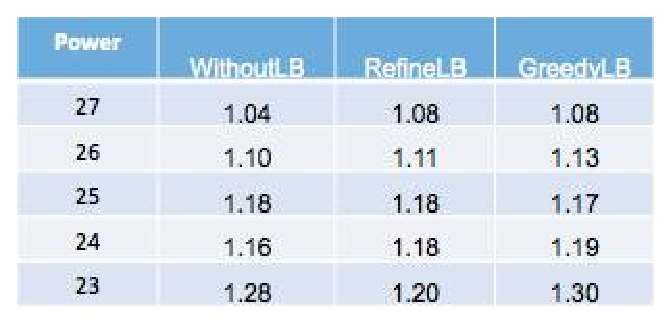
\includegraphics[scale=0.8]{Jacobi/EPS/t2.eps} 
  }
     \end{center}
  \caption{Speedups}
  \label{tb:1}
\end{figure}

There is little or no speed up in cases of higher power caps when using the
power aware load balancer. The reason behind this is the absence of
heterogeneity at higher power caps. The product of object wall time ‘w’ and the
workload ‘x’ comes to be almost the same, and so it leaves power aware LB no
scope of further balancing the workload based on frequency. Load imbalance is
observed only at lower power caps. Hence, there is very little migration that
power aware load balancer does at higher power caps. This makes GreedyLB
perform better at higher power caps, as it takes the greedy approach of freshly
loading the heaviest object with lightest loaded processor. 

GreedyLB and RefineLB are unaware of the differences in frequencies of
different nodes that exist at lower power caps. There is equal weightage given
to each node in GreedyLB and RefineLB. These do not take into account the
frequency of each node and assume that all the nodes in the cluster have
identical performance capability.


\begin{figure}
\centering
  \scalebox{0.75}{
    \begin{tikzpicture}
    \begin{axis}[
     xlabel=  Power Cap Values (W),
     ylabel = Average Idle Time (secs),
     ymax=15, ymin=0, xmax=60, xmin=23,
     x tick label style={black},
     grid=both
     ]
    \addplot table [x=POWER, y= PLB_AV_IDLE]{data.dat};
    \addlegendentry {Power Aware LB}
    \addplot table [x=POWER, y= WOLB_AV_IDLE]{data.dat};
    \addlegendentry {Without LB}
    \addplot table [x=POWER, y= RLB_AV_IDLE]{data.dat};
    \addlegendentry {Refine LB}
    \addplot table [x=POWER, y= GLB_AV_IDLE]{data.dat};
    \addlegendentry {Greedy LB}
    \end{axis}
    \end{tikzpicture}
  }
\caption{Average Idle Time vs Power Comparison between LBs}
\label{fig:avg_times_final_vs_power}
\end{figure}

\begin{figure}
\centering
  \scalebox{0.75}{
    \begin{tikzpicture}
    \begin{axis}[
     xlabel=  Power Cap Values (W),
     ylabel = Max Idle Time (secs),
     ymax=31, ymin=3, xmax=60, xmin=23,
     x tick label style={black},
     grid=both
     ]
    \addplot table [x=POWER, y= PLB_MAX_IDLE]{data.dat};
    \addlegendentry {Power Aware LB}
    \addplot table [x=POWER, y= WOLB_MAX_IDLE_P]{data.dat};
    \addlegendentry {Without LB}
    \addplot table [x=POWER, y= RLB_MAX_IDLE]{data.dat};
    \addlegendentry {Refine LB}
    \addplot table [x=POWER, y= GLB_MAX_IDLE]{data.dat};
    \addlegendentry {Greedy LB}
    \end{axis}
    \end{tikzpicture}
  }
\caption{Max Idle Time vs Power Comparison between LBs}
\label{fig:idle_times_final_vs_power}
\end{figure}


Performance of power aware LB is further analyzed with respect to other LBs in
terms of heterogeneity metrics – average idle time and max idle time, as shown
in Figure \ref{tb:2}. Power aware LB has out performed the other existing power
unaware LBs in terms of average and max idle times. The average idle time is
reduced using the power aware LB by as high as 60\% when compared to the
average idle time of the run without any LB. If compared with RefineLB and
GreedyLB, the reduction is as high as 54\% and 63\% respectively. The average
idle time at 23W comes to be ~12,10,14 and 5sec for runs without LB, with
Refine, Greedy and power aware LBs respectively as shown in figure
\ref{fig:avg_times_final_vs_power}.

\begin{figure}
  \begin{center}
  \scalebox{0.5} {
     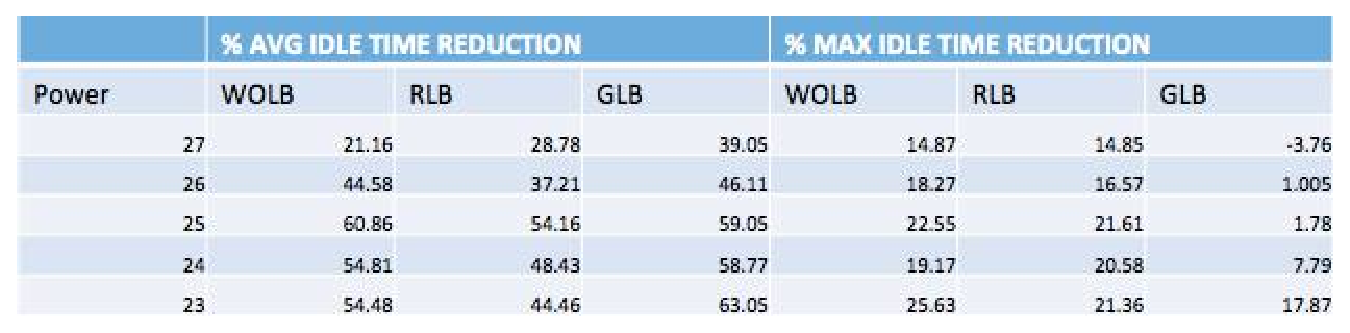
\includegraphics[scale=0.8]{Jacobi/EPS/t1.eps} 
  }
     \end{center}
  \caption{\% Reduction in Idle times}
  \label{tb:2}
\end{figure}

The reduction in maximum idle time is as high as 25\% in the presence of power
aware LB. It is ~30sec in the absence of any load balancer and it comes down to
~23sec when run with power aware LB at a low power cap of 23W as shown in
figure \ref{fig:idle_times_final_vs_power}. We could have further decreased
the maximum idle time. But due to an off node in the cluster with an unexpected
behavior led to an increased max idle time. However average idle time is a
better metric to measure the performance of our load balancer than the max idle
time since it’s taking average idle time into account and the misbehavior by a
one off node doesn’t pull the average down to a great extent unlike the max
idle time metric.

Power aware LB performs equally well in cases of higher power caps when there
is little or no heterogeneity among the nodes. One positive aspect here is that
power aware load balancer does not try to do unnecessary balancing at higher
power caps that could have led to an increase in the average or max idle
leading to an increase in the total execution time.

\begin{figure}
\centering
  \scalebox{0.75}{
    \begin{tikzpicture}
    \pgfplotsset{every axis legend/.append style={
          at={(0.5,1.03)},
          anchor=south}}
    \begin{axis}[
     xlabel=  Core Ids,
     ylabel= Total Execution Time (secs),
     ymax=34, ymin=2, xmax=60, xmin=0,
     x tick label style={black},
     grid=both
     ]
    \addplot table [x=PE, y= PLB]{data1.dat};
    \addlegendentry {With Power Aware LB}
    \addplot table [x=PE, y= RLB]{data1.dat};
    \addlegendentry {With Refine LB}
    \addplot table [x=PE, y= WOLB]{data1.dat};
    \addlegendentry {Without LB}
    \end{axis}
    \end{tikzpicture}
  }
\caption{Heterogeneity comparison between LBs at 23W} 
\label{fig:heter_final}
\end{figure}

Another observation of the total execution time is done on a per core basis at
23W. Figure\ref{fig:heter_final} depicts the amount of heterogeneity among the
nodes. Further from the same figure we can note that there is a lot of
difference in the total execution times by each node in the absence of any load
balancer. The total execution time ranges from 15-35 sec for the run without
any load balancer. RefineLB does not help in minimizing the heterogeneity by a
large extent. The range of total execution times remains close to 15-30 sec.
The power aware load balancer proves to redistribute the workload in a better
manner compared to existing Load Balancers.  As depicted in figure
\ref{fig:heter_final} the range of total execution time has decreased to 15-25
sec with most of the nodes closing to the average. The range could be further
reduced by making use of node specific information or hard coding based on
performance profiling of individual nodes. This profiling information is not
incorporated as they make the load balancer usable only for specific
applications running on known clusters.
